
In order to judge different performance measures of our final model, we require a baseline.
Such a baseline needs to align to the collection of tasks described in Section~\ref{sec:introduction} as close as
possible to allow for good comparability of results.

While there exist multiple machine learning approaches with a setup similar to that of the \ac{vq}
i.e.\ generative models with latent representations such as \ac{gan}, differences in the details make these hard to
compare against each other.
When sticking to the example of \ac{gan} as described by~\cite{gan}, one key difference is that similar to the
\ac{vq} after training the PixelCNN, the latents represent a distribution that is close to that of the training
data, but can not be created by encoding real world data.

\subsection{Autoencoder}\label{subsec:autoencoder}
Since it is the original model that the non-quantized \ac{vae} is based on, which in turn later was developed into the
\ac{vq} and because it also fulfils our requirement of sufficient simplicity, we chose a basic \ac{ae} as our general
baseline method.

A very basic \ac{ae} as described by~\cite{autoenc} and illustrated in Figure~\ref{fig:ae}, is a neural
network that is fed
the
original data, in our case the
image, and then compresses the data down to a lower dimension using one or more hidden and fully connected layers,
the encoding stage.
The result of this encoding stage is fed into a latent layer, whose dimensions decide the size of the compressed
representation.
The output of this latent layer, the actual latent, is than upsampled by a decoding stage, which follows an inverted
structure of the encoding stage.
The output of the net, the reconstruction, is now of the same shape as the input data and can be directly compared
to it.

The model can be trained by applying gradient descent on some form of cost function that describes reconstruction error
like \ac{mse}, theoretically pushing the network to encode the information most important to deconstruction in the
latent.

The similarities to \ac{vq} allow for very comparable results, since the \ac{ae} can be tuned to be very
close in size, training and inference cost.
During implementation of the \ac{ae} baseline, we adhere to the same architecture as the \ac{vq} wherever possible,
exchanging the fully connected layers of the standard \ac{ae} with the downsampling layers and
residual blocks from the \ac{vq} implementation in our reference paper.
This will likely increase its power significantly, as convolutional \ac{ae} have been shown to be superior to the
basic feed-forward \ac{ae} on the realm of image reconstruction by~\cite{convae}.

\begin{figure}[H]
    \centering
    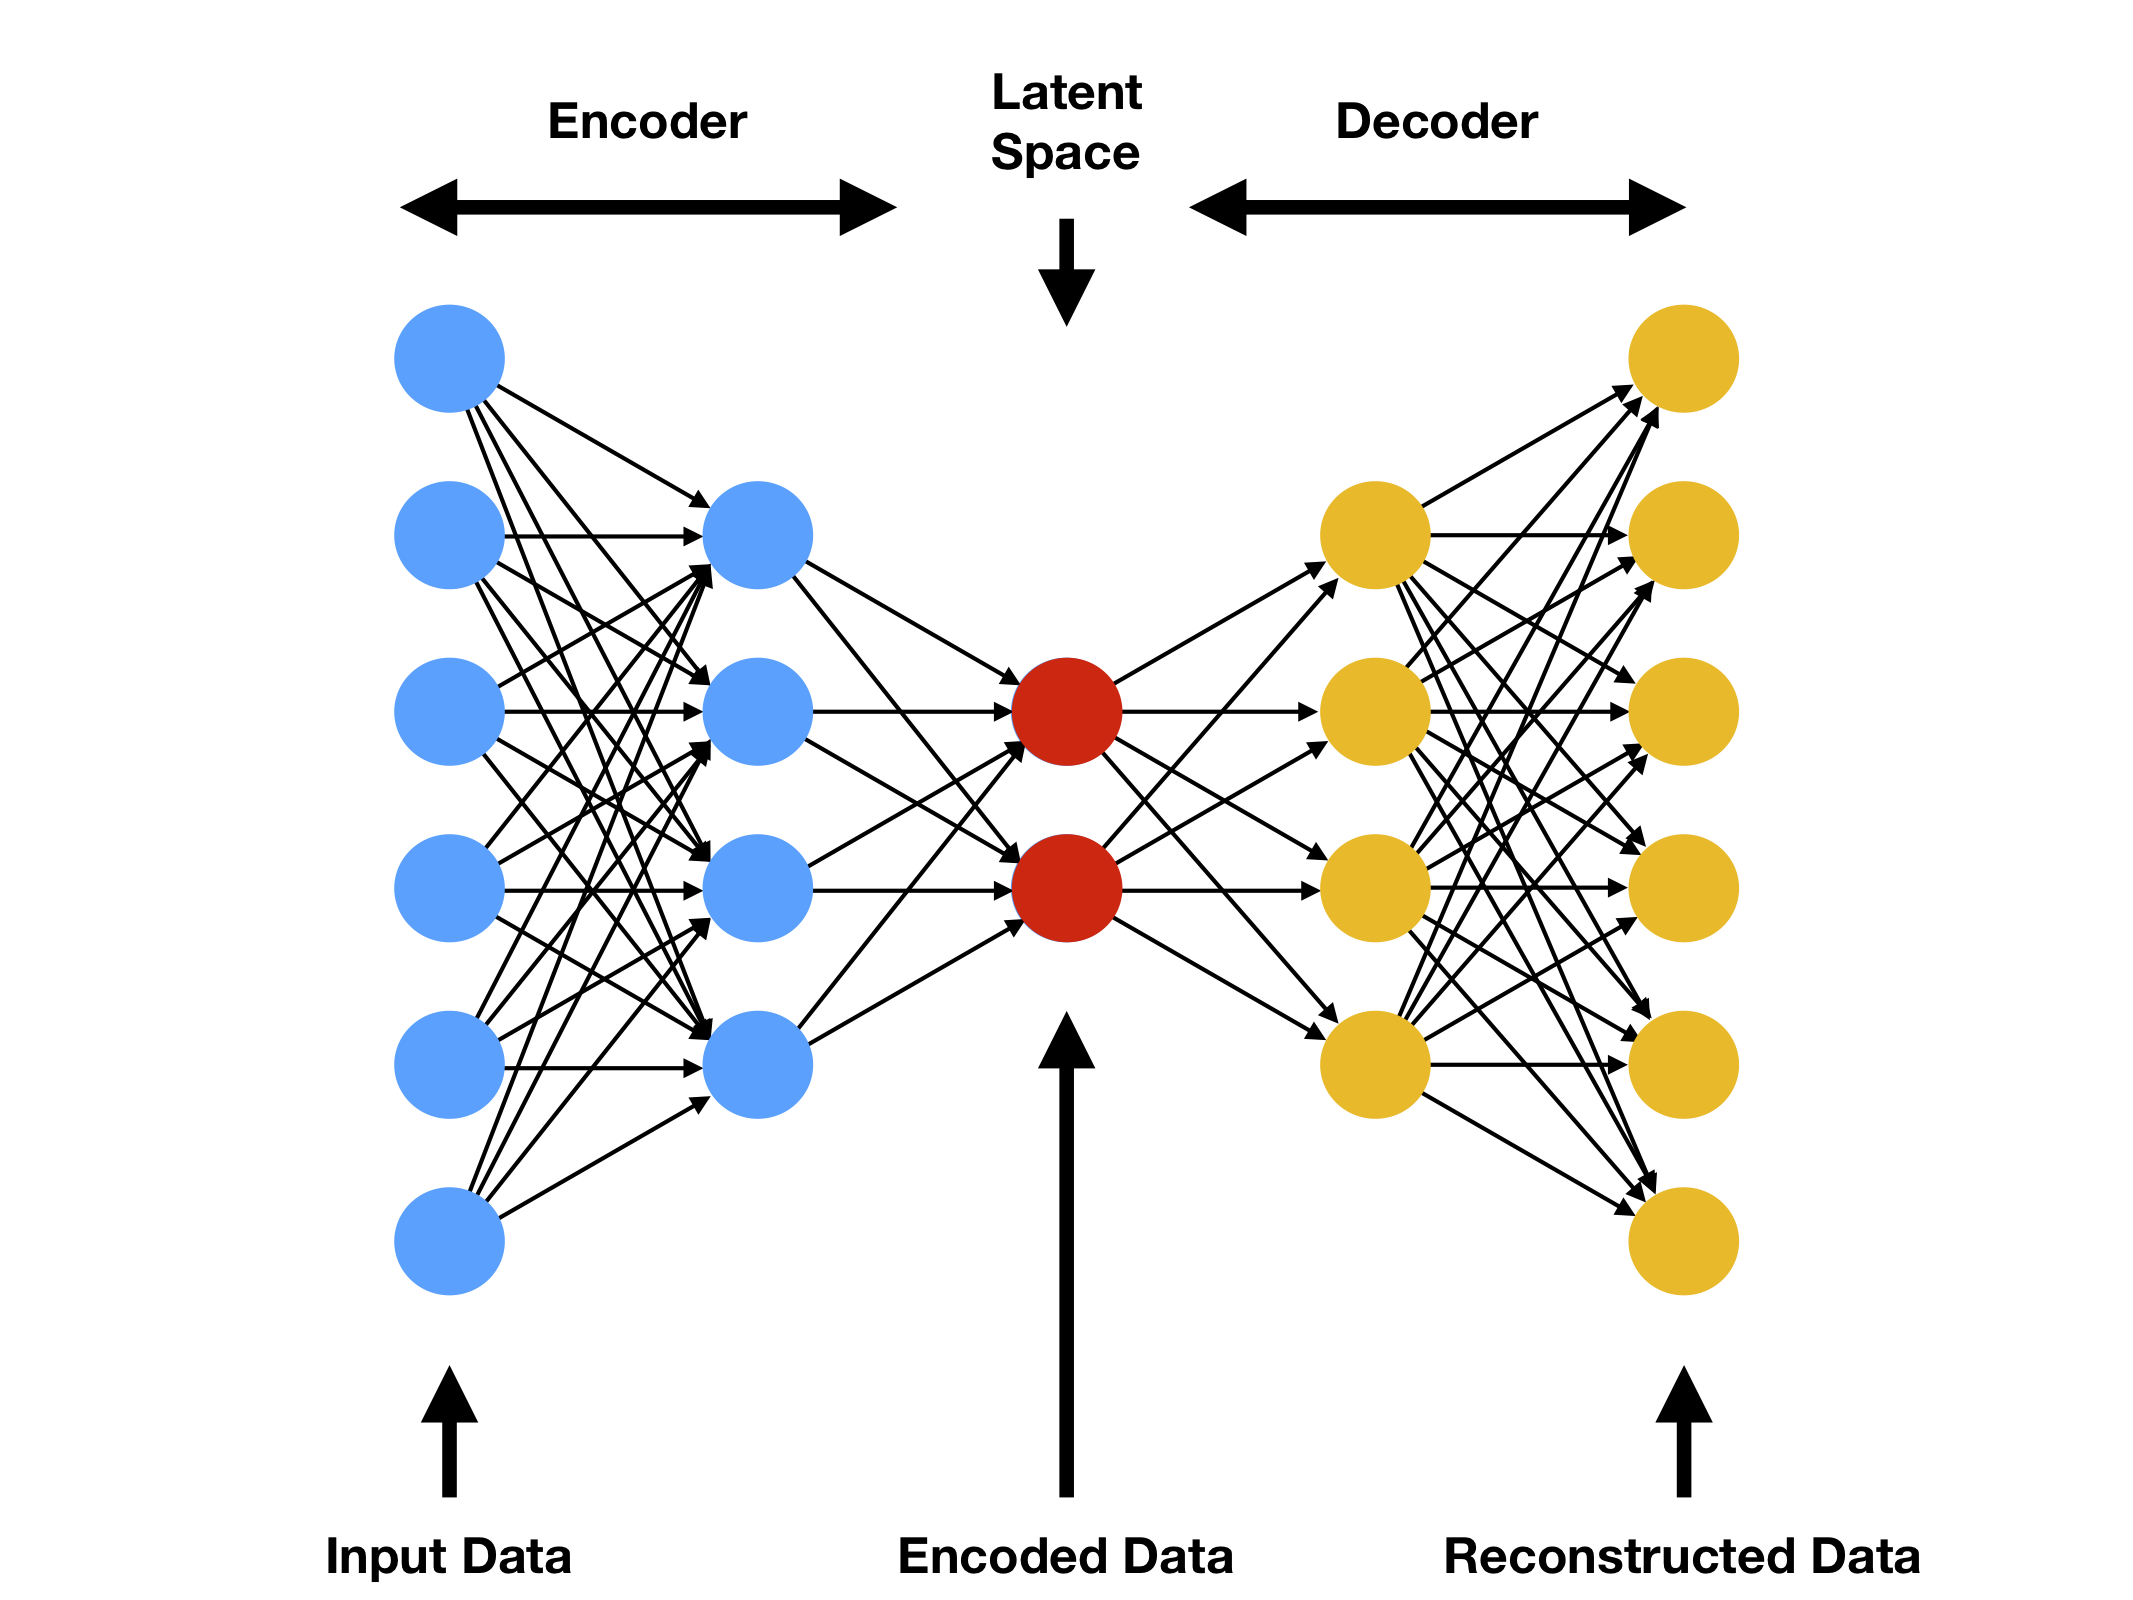
\includegraphics[width=0.7\textwidth]{images/ae}
    \caption{Illustration of a basic \ac{ae} architecture from~\cite{ae_pic}}
    \label{fig:ae}
\end{figure}

\subsection{Variational AE}\label{subsec:variational-ae}
Examining the differences between the different evolutionary steps towards the \ac{vq} could prove to be valuable
for our understanding of its performance.
Therefore, we also implement a \ac{vae}, which substantially differs from the \ac{ae} in the way that latents are
generated.
When constructing the neural network, we follow the same paradigm as with the \ac{ae} before, using the same
encoding and decoding layers as far as possible.
The important difference of the VAE is that its encoder outputs a random variable
$\boldsymbol{\hat{z}} \sim \mathcal{N}(\boldsymbol{\mu_\theta}, \text{diag}
(\boldsymbol{\sigma_\theta}))$. $\boldsymbol{\hat{z}}$ is obtained using the
reparameterization trick, which consists in sampling $\boldsymbol{z}
\sim \mathcal{N}(0, I)$ and then computing $\boldsymbol{\hat{z}} =
\boldsymbol{\mu_\theta} + \boldsymbol{z} \odot \boldsymbol{\sigma_\theta}$.
$\boldsymbol{\mu_\theta}$ and $\boldsymbol{\sigma_\theta}$ are deterministic
outputs of the last convolutional layer of the \ac{vae} encoder.
This allows to optimize the model using the ELBO loss which in turn enables us to not only
reconstruct the input, but to learn a posterior distribution $p(x|z)$ while
the encoder $q(z|x)$ tries to be as close as possible to $p(z)$.
Thus enabling us to generate new dataset samples by sampling $z \sim p(z)$ and then feeding
it through the decoder.
\vskip 1em
\textbf{A Note on Overfitting:}
Overfitting refers to the phenomenon where a model starts to memorize the training data instead of learning useful
features from the training data that generalize well to unseen data as is the goal.

While theoretically, this may very well be an issue with \ac{ae} and \ac{vae}, we have not experienced this happening
yet with either when training with adequate training-set sizes.
This is very likely due to the large dataset size and the inductive bias of the convolution operation~\cite{citationNeeded}.

\subsection{Non-ML Baseline: JPEG}\label{subsec:jpeg}
While much of the current work in realistic high resolution image generation is based on \ac{dnn}~\cite{citationNeeded},
the field of image compression is well researched both in-, and outside deep architectures~\cite{compression},
and non-ML approaches are still dominant on the web as can be seen in Figure~\ref{fig:file_formats}.
To represent this, we also use the popular JPEG format for comparisons against our lossy compression schemes.

\begin{figure}[H]
    \centering
    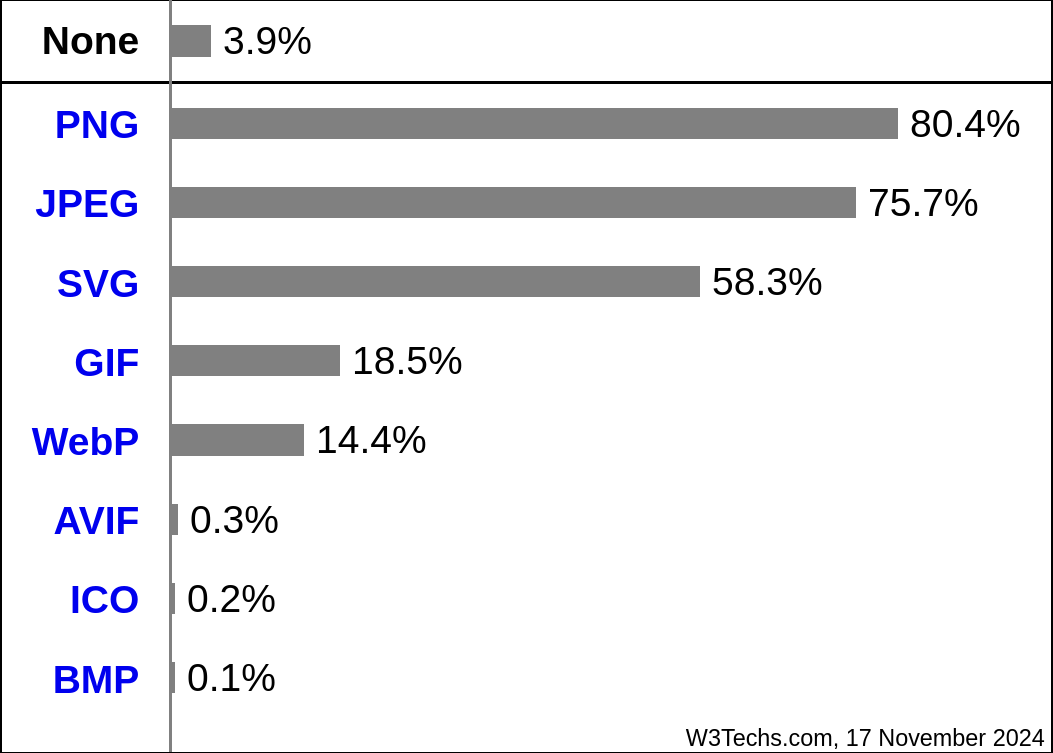
\includegraphics[width=0.5\textwidth]{images/formats}
    \caption{Percentages of websites using various image file formats~\cite{img_file_format}}
    \label{fig:file_formats}
\end{figure}